
\chapter{The Steganos Project}
\begin{multicols*}{2}
Steganos is the name of the application that implements the algorithms enumerated in the earlier chapters of this paper and is the direct result of the work done by the authors. In this chapter I will present what modern technologies and frameworks went into creating the application, how it is structured from an Object Oriented point of view, how fast it is and how I hope it will expand into the future.

\section{Used technologies}
\subsection{C++}
C++ is one of the lowest high-level computer programming languages. Designed by Bjarne Stroustrup, it first appeared in 1985 as a variation of one of the most popular languages at the time, C. It is one of the most efficient modern languages mainly because it has been designed with performance and flexibility in mind, just like its predecessor. C++ has gained a lot of traction  from big companies like Intel and Microsoft which needed a programming language that could be used for operations ranging from basic kernel functions to highly specialized Object-Oriented projects with Graphical User Interfaces\cite{stroustrup_2018}.

Since its conception, C++ has grew substantially by adding support for generic and functional features to ease the development processes and getting standardized by the International Organization for Standardization probably helped as well because it meant no more obscure variations of the language, allowing programmers to follow only one standard, ending up with even more portability and stability of the applications.

In the modern day, it is used almost everywhere: the kernel of various operating systems, the transaction software used by banks, drones and airplanes, embedded systems such as the Arduino or Raspberry Pi, and now in the Steganos Project as well under the latest approved standard of the language, C++17.

C++ inherited from C the file types: headers and sources. The header files (the files that have a .h or .hpp extension) are where the standard recommends to store the class declarations, function prototypes, constants declarations, no definitions should take place in a header file. There are a few exceptions to this rule, the most common one being a rule that states that all templated functions and functions are to be declared and defined in a header file otherwise it will not work properly when dealing with multiple instances of different types. In the case of the source files (the files that have the .c or .cpp extension) the standard suggests to only be used for the definition of the class methods or other general functions. Following the standard results most of the time in a clean and well defined separation in the code, allowing for high cohesion and low coupling in all projects built using C++.

The reason for choosing C++ as the language for the Steganos project is simple: it allows for the programmer to work on the raw bytes of files in an extremely easy way, reading and parsing them, bit-wise operations and writing to file, all the common low-level operations that are highly valued when working in the steganography field. But the high level aspects of the language also permit for dealing with complex tasks, such as modern cryptography algorithms applied to robust byte streams or holding all the information in different data structures.

\subsection{CMake}
CMake is a cross-platform open-source tool designed for managing the build process of software based on the C++ programming language. It has been created in the year 2000 and ever since then it stayed compiler-independent using simple configuration files that generate the adequate makefiles to be used in the users environment while building the target project\cite{cmake}.

CMake uses files called CMakeLists.txt that contain the commands to be used by the internals of the tool in the building process. It is required that one file is in the root of the project before running the CMake process, with the possibility of adding a .txt file in the subdirectories in order to indicate special cases that require a different approach.

\begin{figure}[H]
    \centering
    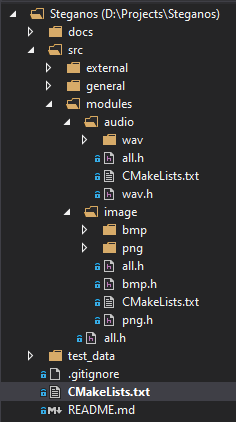
\includegraphics[height=6.9cm,keepaspectratio]{pics/cmake_folder_structure_example}
    \caption{Folder structure of a project using CMake}
\end{figure}

Each command in CMake has the same format: COMMAND (args..). Using this format, users are able to build even the most complex software projects in the form of simple executables, dynamic or static linked libraries, etc. Steganos uses CMake because it is an extremely effective tool in the building process and it allows for separating the logic of the project into distinct modules i.e. the audio module, the image module, the general usage module, and linking them in the end into a simple executable. Most projects use only a small subset of the commands available in CMake, the most common being:

\begin{itemize}
  \item \textbf{CMAKE\_MINIMUM\_REQUIRED} is used to mark the minimum version of CMake that is required to be installed on a system in order to build the project.
  \item \textbf{SET} is used to assign a value to a CMake variable that is used while building, similar to environment variables found on all operating systems.
  \item \textbf{PROJECT} for naming the project, important step in active Continous Integration and Continous Development environments.
  \item \textbf{INCLUDE\_DIRECTORIES} for marking the directories containing the header files in order for the compiler to be able to link the source files and header files.
  \item \textbf{ADD\_EXECUTABLE} for creating an executable after build the project from the source files given as arguments.
  \item \textbf{ADD\_LIBRARY} for creating a library or module with the given source files.
  \item \textbf{TARGET\_LINK\_LIBRARIES} for linking (pre)defined modules or executables between eachother.
\end{itemize}


\subsection{CXXOpts}
CXXOpts is an open-source C++ library that is meant to be a lightweight command line option parser\cite{jarro2783_2020}. It is meant as the C++11 and beyond alternative to other libraries such as Commons CLI for Java or Argparse for Python. It was initially created by user jarro2783 on Github and nowadays is actively developed by the community using the Git commit and pull request system. CXXOpts is made to replicate the handling of the help argument and the merging of multiple parameters commonly found in *NIX command line binaries, without using any additional dependencies in a header-only file.


\subsection{Lodepng}
Lodepng is an open source C++ library developed by Lode Vandevenne used for image processing for pictures stored under the PNG format \cite{lvandeve_2020}. It is very useful for decoding the image data before beginning the steganography process, making it easy to modify the data and to encode it back into a PNG file that follows the standard format. Lodepng works on every version of C++, contains only two files(a source file and a header file) and is rated to be one of the fastest libraries for PNG image processing. Steganos uses Lodepng to parse PNG files and to obtain the image data byte stream from the zlib compressed stream in order to be able to work with the implemented steganographic algorithms.

\subsection{MMSSTV Engine for Windows}

\subsection{Robot36 for *NIX based systems}

\section{Application architecture}

\section{Benchmarks}

\section{Further work}
\end{multicols*}